%%%%%%%%%%%%%%%%%%%%%%%%%%%%%%%%%%%%%%%%%%%%%%%%%%%%%%%%%%%%%%%%%%%%%%
% Lớp 11 | Đường thẳng, mặt phẳng. Quan hệ song song trong | Hai mặt phẳng song song
% Dạng 1H4?4-1: Câu hỏi lý thuyết
% Số câu: 32  (sinh tự động bởi tach_cau.py; từ nay thầy sửa trực tiếp file này)
%%%%%%%%%%%%%%%%%%%%%%%%%%%%%%%%%%%%%%%%%%%%%%%%%%%%%%%%%%%%%%%%%%%%%%

%%%%%%%%%%%%%%%% TRẮC NGHIỆM 4 PHƯƠNG ÁN %%%%%%%%%%%%%%%%

% nguồn: Ok_Toan11_TracNghiem_Lan2
\begin{ex}%[1H4N4-1]%[ma:fd2e20e2]
	Cho hình lăng trụ $ABC.A'B'C'$. Gọi $I$, $J$, $K$ lần lượt là trọng tâm của các tam giác $ABC$,  $ACC'$, $A'B'C'$ như hình vẽ. Mặt phẳng nào sau đây song song với mặt phẳng $\left(IJK\right)$?
	 \choice
		 {$\left(ABB'\right)$}
		{$\left(ACC'\right)$} 
		 {$\left(ABC'\right)$}
		 {\True $\left(BB'C'\right)$}
	\loigiai{ 
		\begin{center}
			\begin{tikzpicture}[scale=0.8,font=\footnotesize,line join=round,line cap=round,>=stealth]
					\coordinate (A) at (-2,0); 
					\coordinate (B)  at (-1,-2);
					\coordinate  (C) at (2,0);
					\coordinate (H) at (1,4); 
					\foreach \i in {A,B,C}{\coordinate (\i') at ($(\i)+(H)$); \draw (\i)--(\i');} 
					\draw (A')--(B')--(C')--cycle; 
					 \draw (A)--(B)--(C);
					\draw[dashed,thin](A)--(C); 
					\coordinate (M)  at ($(B)!0.5!(C)$);
					\coordinate (N) at  ($(B')!0.5!(C')$);
					\coordinate (P)  at ($(C')!0.5!(C)$);
					 \coordinate (I) at ($(A)!0.67!(M)$);
					\coordinate  (K) at ($(A')!0.67!(N)$);
					\coordinate  (J) at ($(A)!0.67!(P)$); A
					 \draw (A')--(N);
					\draw[dashed,thin](A)--(M) 
						(A)--(P) 
						(I)--(K)--(J)--(I); 
					 \foreach \i/\g in {A/180,B/-90,C/0,A'/180,B'/180,C'/0,I/-90,K/60,J/60}{\draw[fill=black](\i) circle (1pt)
						($(\i)+(\g:4mm)$) node[scale=1]{$\i$};} 
				\end{tikzpicture}
		\end{center}
		Dựa vào quan hệ  song song ta có $\left(IJK\right)\parallel \left(BCC'B'\right)$ suy ra $\left(IJK\right)\parallel \left(BB'C'\right)$.
	 }
\end{ex}

% nguồn: Ok_Toan11_TracNghiem_Lan2
\begin{ex}%[1H4N4-1]%[ma:4955646e]
	Trong các  khẳng định sau, khẳng định nào đúng?
	 \choice
		{Qua  một điểm có vô số mặt phẳng song song với một mặt phẳng cho trước}
		{Qua một điểm nằm ngoài một mặt phẳng, có vô  số mặt phẳng song song với mặt phẳng đã cho}
		{\True Qua một điểm nằm ngoài một mặt phẳng, tồn tại  duy nhất một mặt phẳng song song với mặt phẳng đã cho}
		{Qua một  điểm tồn tại duy nhất một mặt phẳng song song với một mặt phẳng cho trước}
	 \loigiai{
		Qua một điểm nằm ngoài  một mặt phẳng, có một và chỉ một mặt phẳng song song với mặt phẳng đó.
	 }
\end{ex}

% nguồn: Ok_TracNghiemLop11_Lan1
\begin{ex}%[1H4N4-1]%[ma:acd4164a]
	Hãy chọn  mệnh đề đúng trong các mệnh đề sau đây?
	 \choice
		{Hình lăng trụ có tất  cả các mặt là hình bình hành}
		{Nếu hai mặt phẳng $(P)$ và $(Q)$ lần  lượt chứa hai đường thẳng song song thì song song với nhau}
		{Qua một điểm tồn  tại duy nhất một mặt phẳng song song với một mặt phẳng cho trước}
		{\True Qua một điểm nằm ngoài một mặt phẳng, tồn tại duy nhất một  mặt phẳng song song với mặt phẳng đã cho}
	\loigiai{ 
		 Dựa vào tính chất ta có mệnh đề \lq\lq Qua một điểm nằm ngoài một mặt phẳng, tồn tại duy nhất một mặt phẳng song song với mặt phẳng đã cho\rq\rq~là mệnh đề đúng.
	 }
\end{ex}

% nguồn: Ok_TracNghiemLop11_Lan1
\begin{ex}%[1H4N4-1]%[ma:27393b6e]
	Cho hai mặt phẳng song song $(\alpha)$ và $(\beta)$.  Đường thẳng $a$ nằm trong mặt phẳng $(\alpha)$ và đường thẳng $b$ nằm trong mặt phẳng $(\beta)$. Khẳng định nào sau đây \textbf{sai}?
	 \choice
		{$a \parallel  (\beta)$}
		 {$b \parallel (\alpha)$}
		{\True $a  \parallel b$}
		{Nếu tồn tại mặt phẳng $\gamma  $ chứa cả hai đường thẳng $a$ và $b$ thì $a \parallel b$}
	 \loigiai{
		Mệnh đề \lq\lq $a \parallel b$\rq\rq\ là sai vì chúng  có thể chéo nhau.
	} 
\end{ex}

% nguồn: Ok_TracNghiemLop11_Lan1
\begin{ex}%[1H4N4-1]%[ma:e10c152c]
	Tìm khẳng định {\bfseries sai} trong các khẳng định sau đây? 
	\choice 
		{Nếu  hai mặt phẳng song song cùng cắt mặt phẳng thứ ba thì hai giao tuyến tạo thành song song với nhau}
		{Ba mặt phẳng đôi một song song chắn trên hai  đường thẳng chéo nhau những đoạn thẳng tương ứng tỉ lệ}
		{Nếu mặt phẳng $(P)$ song song  với mặt phẳng $(Q)$ thì mọi đường thẳng nằm trên mặt phẳng $(P)$ đều song song với mặt phẳng $(Q)$}
		{\True Nếu mặt phẳng $(P)$ có chứa hai đường thẳng phân biệt và hai đường thẳng đó cùng song  song song với mặt phẳng $(Q)$ thì mặt phẳng $(P)$ song song với mặt phẳng $(Q)$}
	 \loigiai{
	``Nếu mặt phẳng $(P)$ có chứa hai đường thẳng phân biệt và hai đường thẳng đó cùng song song song với mặt phẳng $(Q)$  thì mặt phẳng $(P)$ song song với mặt phẳng $(Q)$'' là mệnh đề sai khi hai đường thẳng đó song song với nhau.}
\end{ex}

% nguồn: Ok_TracNghiemLop11_Lan1
\begin{ex}%[1H4N4-1]%[ma:057faa5b]
	Quan hệ song song trong không gian có tính chất nào trong  các tính chất sau?
	\choice 
		{\True Nếu hai mặt phẳng $(P)$ và $(Q)$ song song với nhau thì mọi đường  thẳng nằm trong $(P)$ đều song song với $(Q)$}
		{Nếu hai mặt phẳng $(P)$ và $(Q)$ song song với nhau thì mọi đường thẳng nằm trong $(P)$ đều song song với mọi đường  thẳng nằm trong $(Q)$}
		{Nếu hai đường thẳng song song với  nhau lần lượt nằm trong hai mặt phẳng phân biệt $(P)$ và $(Q)$ thì $(P)$ và $(Q)$ song song với nhau}
		{Qua  một điểm nằm ngoài mặt phẳng cho trước ta vẽ được một và chỉ một đường thẳng song song với mặt phẳng cho trước đó}
	 \loigiai{
		Ta thấy  tính chất
		\begin{itemize}
			\item Nếu hai mặt phẳng $(P)$ và $(Q)$ song song với nhau thì mọi đường thẳng nằm trong $(P)$  đều song song với $(Q)$ là đúng.
			\item Nếu hai mặt phẳng $(P)$ và $(Q)$ song song với  nhau thì mọi đường thẳng nằm trong $(P)$ đều song song với mọi đường thẳng nằm trong $(Q)$ là sai vì có thể xảy ra hai đường thẳng chéo nhau.
			\item Nếu hai đường thẳng song song với nhau lần lượt nằm trong hai mặt phẳng phân biệt $(P)$ và $(Q)$ thì $(P)$ và $(Q)$ song song với nhau là sai theo tính chất  thì phải là hai đường thẳng cắt nhau.
			\item Qua một điểm nằm ngoài mặt phẳng cho trước ta vẽ được một và chỉ một đường thẳng song song với mặt phẳng cho trước đó là sai vì có thể vẽ được vô số các đường thẳng. 
		\end{itemize}
	 }
\end{ex}

% nguồn: Ok_TracNghiemLop11_Lan1
\begin{ex}%[1H4N4-1]%[ma:b9cc154c]
	Điều kiện cần và đủ để hai mặt  phẳng song song với nhau là
	 \choice
		 {Hai mặt phẳng đó cùng song song với một mặt phẳng thứ ba}
		{Hai mặt  phẳng đó cùng song song với một đường thẳng}
		{\True Hai mặt phẳng  đó không có điểm chung}
		{Có một mặt  phẳng chứa hai đường thẳng phân biệt cùng song song với mặt phẳng còn lại}
	\loigiai{ 
		Điều kiện cần và đủ để hai  mặt phẳng song song với nhai là hai mặt phẳng đó không có điểm chung.
	 }
\end{ex}

% nguồn: Ok_TracNghiemLop11_Lan1
\begin{ex}%[1H4N4-1]%[ma:1868d89e]
	Mệnh đề nào dưới  đây là đúng?
	\choice 
		{Qua một điểm nằm ngoài mặt phẳng cho trước, ta vẽ được một và chỉ một đường thẳng song  song với mặt phẳng cho trước đó}
		{Nếu hai mặt phẳng $\left( \alpha \right)$  và $\left( \beta \right)$ song song với nhau thì mọi đường thẳng nằm trong mặt phẳng $\left( \alpha \right)$ đều song song với mọi đường thẳng nằm trong mặt phẳng $\left( \beta \right)$}
		{Nếu hai đường thẳng song song với nhau lần lượt nằm trong hai mặt phẳng phân biệt $\left( \alpha \right)$ và $\left( \beta \right)$ thì $\left( \alpha \right)$  và $\left( \beta \right)$ song song với nhau}
		{\True Nếu hai mặt phẳng $\left( \alpha \right)$ và $\left( \beta \right)$ song song với nhau thì mọi đường thẳng nằm trong mặt phẳng $\left(  \alpha \right)$ đều song song với mặt phẳng $\left( \beta \right)$}
	\loigiai{ 
		Nếu hai mặt phẳng $\left( \alpha \right)$ và $\left( \beta \right)$ song song với nhau  thì mọi đường thẳng nằm trong mặt phẳng $\left( \alpha \right)$ đều song song với mặt phẳng $\left( \beta \right)$
	} 
\end{ex}

% nguồn: Ok_TracNghiemLop11_Lan1
\begin{ex}%[1H4N4-1]%[ma:f9e2bcc0]
	Cho các  mệnh đề sau
	\begin{enumerate}[1.]
		\item Hai mặt phẳng cùng song song với một mặt phẳng thứ ba thì chúng song  song với nhau.
		\item Hai mặt phẳng phân biệt cùng song song với một đường thẳng thì  chúng song song với nhau.
		\item Bất kì đường thẳng nào cắt một trong hai mặt phẳng song song thì nó cũng  cắt mặt phẳng còn lại.
	\end{enumerate}
	Số  mệnh đề $\textbf{sai}$ là
	\choice 
		{$0$} 
		{$3$} 
		 {$1$}
		{\True  $2$}
	 \loigiai{
		\begin{enumerate}[+]
			\item Mệnh đề \lq\lq Hai mặt phẳng phân biệt cùng song song với một đường thẳng thì chúng song song với nhau\rq\rq\ là một mệnh đề sai vì chúng có thể cắt  nhau.
			\item Mệnh đề \lq\lq Hai mặt phẳng cùng song song với một mặt phẳng thứ ba thì chúng song song với nhau\rq\rq\ là một  mệnh đề sai vì hai mặt phẳng này có thể trùng nhau.
			\item Mệnh đề \lq\lq Bất kì đường thẳng nào cắt một trong hai mặt phẳng song song thì nó cũng cắt  mặt phẳng còn lại\rq\rq\ là một mệnh đề đúng.
		\end{enumerate}
		Vậy có hai mệnh đề  sai.
	} 
\end{ex}

% nguồn: Ok_Toan11_TracNghiem_Lan2
\begin{ex}%[1H4H4-1]%[ma:eb692f61]
	Trong các  mệnh đề dưới đây, mệnh đề nào đúng?
	\choice 
		{\True Nếu hai mặt phẳng $\left(\alpha\right)$ và $\left(\beta\right)$ song song với  nhau thì mọi đường thẳng nằm trong $\left(\alpha\right)$ đều song song với $\left(\beta\right)$}
		{Nếu hai mặt phẳng $\left(\alpha\right)$ và $\left(\beta\right)$ song song với nhau thì bất kì đường thẳng nào nằm trong $\left(\alpha\right)$ cũng song song với bất kì đường thẳng nào  nằm trong $\left(\beta\right)$}
		{Nếu hai đường thẳng phân biệt $a$ và $b$ song song lần lượt nằm trong hai mặt phẳng $\left(\alpha\right)$ và $\left(\beta\right)$  phân biệt thì $\left(\alpha\right)\parallel \left(\beta\right)$}
		{Nếu đường thẳng $d$ song song với mặt  phẳng $\left(\alpha\right)$ thì nó song song với mọi đường thẳng nằm trong $\left(\alpha\right)$}
	\loigiai{ 
	Mệnh đề: ``Nếu hai mặt phẳng $\left(\alpha\right)$ và $\left(\beta\right)$ song song với  nhau thì mọi đường thẳng nằm trong $\left(\alpha\right)$ đều song song với $\left(\beta\right)$.'' là đúng.}
\end{ex}

% nguồn: Ok_Toan11_TracNghiem_Lan2
\begin{ex}%[1H4H4-1]%[ma:11b343da]
	 Tìm mệnh đề đúng trong các mệnh đề sau đây:
	 \choice
		{\True Nếu hai mặt phẳng $\left(\alpha\right)$ và  $\left(\beta\right)$ song song với nhau thì mọi đường thẳng nằm trong $\left(\alpha\right)$ đều song song với $\left(\beta\right)$}
		{Nếu hai mặt  phẳng $\left(\alpha\right)$ và $\left(\beta\right)$ song song với nhau thì mọi đường thẳng nằm trong $\left(\alpha\right)$ đều song song với mọi đường thẳng nằm trong $\left(\beta\right)$}
		{Nếu hai đường thẳng song song với nhau lần lượt nằm  trong hai mặt phẳng phân biệt $\left(\alpha\right)$ và $\left(\beta\right)$ thì $\left(\alpha\right)$ và $\left(\beta\right)$ song song với nhau}
		{Qua  một điểm nằm ngoài mặt phẳng cho trước có một và chỉ một đường thẳng song song với mặt phẳng cho trước đó}
	 \loigiai{
		Nếu hai mặt phẳng $\left(\alpha\right)$ và $\left(\beta\right)$ song song với  nhau thì mọi đường thẳng nằm trong $\left(\alpha\right)$ đều song song với $\left(\beta\right)$.
	} 
\end{ex}

% nguồn: Ok_Toan11_TracNghiem_Lan2
\begin{ex}%[1H4H4-1]%[ma:38fe1c62]
	Cho hình hộp $ABCD.A'B'C'D'$. Gọi $O$, $O'$ lần lượt là tâm của hai đáy $ABCD$ và $A'B'C'D'$. Mệnh đề nào  sau đây sai?
	\choice 
		{\True  $\left(BA'D'\right) \parallel \left(ADC'\right)$}
		{$\left(ABB'\right) \parallel \left(CDD'\right)$} 
		{$\left(ABO'\right)  \parallel \left(OC'D'\right)$}
		{$\left(B'AC\right) \parallel \left(DA'C'\right)$} 
	\loigiai{ 
		\begin{center}
			\begin{tikzpicture}[scale=0.8,font=\footnotesize,line join=round,line cap=round,>=stealth]
					\coordinate (B) at  (0,0);
					\coordinate (A) at (-2,-2); 
					\coordinate (C) at  (6,0);
					 \coordinate (D) at ($(A)+(C)-(B)$);
					\foreach \i in {A,B,C,D}{\coordinate  (\i') at ($(\i)-(0,4)$);}
					\coordinate  (O) at ($(A)!0.5!(C)$); C
					\coordinate  (O') at ($(A')!0.5!(C')$);
					\draw  (A)--(B)--(C)--(D)--cycle;
					\draw (A)--(A') 
						 (C)--(C')
						(D)--(D') 
						 (A')--(D')--(C')
						(B)--(D) 
						(A)--(C); 
					\draw[dashed,thin] (B)--(B')--(A') 
						 (B')--(C')
						 (A')--(C')
						 (B')--(D');
					\foreach  \i/\g in {A'/170,B'/170,C'/-90,D'/-90,A/90,B/90,C/-20,D/10,O/120,O'/120}{\draw[fill=blue](\i) circle (1pt)
						($(\i)+(\g:5mm)$) node[scale=1]{$\i$};} 
				\end{tikzpicture}
		\end{center}
		Ta có $\left(BA'D'\right) \parallel \left(ADC'\right)$ là mệnh đề sai. 
	} 
\end{ex}

% nguồn: Ok_Toan11_TracNghiem_Lan2
\begin{ex}%[1H4H4-1]%[ma:13158493]
	Cho hai mặt phẳng song song $\left(\alpha\right)$ và  $\left(\beta\right)$, đường thẳng $a\parallel \left(\alpha\right)$. Có bao nhiêu vị trí tương đối của $a$ và $\left(\beta\right)$?
	 \choice
		{$1$} 
		{\True $2$} 
		{$3$} 
		 {$4$}
	 \loigiai{
		 Vì $\heva{
		&\left(\alpha\right)\parallel \left(\beta\right)\\ 
		& a\,\parallel \left(\alpha\right)}$ nên $a$ và $\left(\beta\right)$ chỉ có thể có $2$ vị trí tương đối $\left(\alpha\right)\parallel \left(\beta\right)$ hoặc $a$  nằm trên $\left(\beta\right)$.
	} 
\end{ex}

% nguồn: Ok_Toan11_TracNghiem_Lan2
\begin{ex}%[1H4H4-1]%[ma:a59d207f]
	Trong các điều kiện sau, điều  kiện nào kết luận $\left(\alpha\right)\parallel\left(\beta\right)$?
	 \choice
		 {\True $\left(\alpha\right)\parallel a$ và $\left(\alpha\right)\parallel b$ với $ a$, $b$ là hai đường thẳng cắt nhau thuộc $\left(\beta\right)$}
		{$\left(\alpha\right)\parallel  a$ và $\left(\alpha\right)//b$ với $ a$, $b$ là hai đường thẳng phân biệt thuộc $\left(\beta\right)$}
		{$\left(\alpha\right)\parallel a$ và $\left(\alpha\right)\parallel b$ với $ a$, $b$ là hai đường thẳng phân biệt cùng song song với $\left(\beta\right)$} 
		{$\left(\alpha\right)\parallel\gamma $ và $\left(\beta\right)\parallel\left(\gamma\right)$  với $\left(\gamma\right)$ là mặt phẳng nào đó}
	 \loigiai{
		Ta có $\heva{&a\parallel\left(\alpha\right)\\&b\parallel\left(\alpha\right)\\& 
		 a,\,b \subset \left(\beta\right)}
	\Rightarrow\left(\alpha\right)\parallel\left(\beta\right)$.} 
\end{ex}

% nguồn: Ok_Toan11_TracNghiem_Lan2
\begin{ex}%[1H4H4-1]%[ma:ead58e3c]
	Cho một đường thẳng $a$ song song  với mặt phẳng $(P)$. Có bao nhiêu mặt phẳng chứa $a$ và song song với $(P)$?
	\choice 
		 {$0$}
		{\True  $1$}
		{$2$} 
		 {Vô số}
	 \loigiai{
	Có duy nhất  một mặt phẳng chứa $a$ và song song với $(P)$.}
\end{ex}

% nguồn: Ok_Toan11_TracNghiem_Lan2
\begin{ex}%[1H4H4-1]%[ma:53891ebb]
	Cho  các mệnh đề sau:
	\begin{enumerate}[1)]
		\item Hai mặt phẳng phân biệt cùng song song với một đường thẳng thì chúng song song  với nhau.
		\item Hai mặt phẳng cùng song song với một mặt phẳng thứ  ba thì chúng song song với nhau.
		\item Bất kì đường thẳng nào cắt một trong hai mặt phẳng song song thì  nó cũng cắt mặt phẳng còn lại.
	\end{enumerate}
	Số mệnh  đề \textbf{sai} là
	\choice 
		 {$0$}
		 {$1$}
		 {$3$}
		 {\True $2$}
	 \loigiai{
		Mệnh đề ``Hai  mặt phẳng phân biệt cùng song song với một đường thẳng thì chúng song song với nhau.'' là một khẳng định sai vì chúng có thể cắt nhau.\\
		Mệnh đề ``Hai mặt  phẳng cùng song song với một mặt phẳng thứ ba thì chúng song song với nhau.'' là một mệnh đề sai vì hai mặt này có thể trùng nhau.\\
		Mệnh đề ``Bất kì đường thẳng nào cắt một trong hai mặt phẳng song song thì nó cũng cắt mặt phẳng còn lại.'' là một mệnh  đề đúng.
	 }
\end{ex}

% nguồn: Ok_Toan11_TracNghiem_Lan2
\begin{ex}%[1H4H4-1]%[ma:888a928b]
	Cho hình hộp $ABCD.A'B'C'D'$. Khẳng  định nào sau đây là sai?
	\choice 
		{\True $\left(BDD'B'\right) \parallel  \left(ACC'A'\right)$}
		{$\left(ABCD\right)  \parallel \left(A'B'C'D'\right)$}
		{$\left(ABB'A'\right) \parallel  \left(CDD'C'\right)$}
		{$\left(AA'D'D\right) \parallel \left(BCC'B'\right)$} 
	 \loigiai{
		Ta thấy  $\heva {\left(ABCD\right) &\parallel \left(A'B'C'D'\right) \\ \left(AA'D'D\right) &\parallel \left(BCC'B'\right) \\ \left(ABB'A'\right) &\parallel \left(CDD'C'\right)}$ luôn đúng và hai mặt phẳng $\left(BDD'B'\right),\left(ACC'A'\right)$ là cắt nhau.
	 }
\end{ex}

% nguồn: Ok_Toan11_TracNghiem_Lan2
\begin{ex}%[1H4H4-1]%[ma:df45606a]
	Cho hai mặt phẳng song song $\left(\alpha\right)$ và $\left(\beta\right)$, $a$ là đường thẳng bất kì. Tìm  mệnh đề \textbf{sai} trong các mệnh đề sau:
	\choice 
		 {Nếu $a$ cắt mặt phẳng $\left(\alpha\right)$ thì $a$ cắt mặt phẳng $\left(\beta\right)$}
		{Nếu $a\subset\left(\alpha\right)$ thì $a$ song song với mặt phẳng $\left(\beta\right)$} 
		{Nếu $a\subset\left(\beta\right)$ thì $a$ song song với  mặt phẳng $\left(\alpha\right)$}
		{\True Nếu $a$  song song với mặt phẳng $\left(\alpha\right)$ thì $a$ song song với mặt phẳng $\left(\beta\right)$}
	\loigiai{ 
		Nếu $a$ song song với mặt phẳng $\left(\alpha\right)$ thì $a$ song song với mặt  phẳng $\left(\beta\right)$.
	 }
\end{ex}

% nguồn: Ok_Toan11_TracNghiem_Lan2
\begin{ex}%[1H4H4-1]%[ma:68ced2cc]
	Chọn khẳng định  \textbf{sai}.
	 \choice
		 {Hai mặt phẳng song song thì mọi đường thẳng nằm trên mặt phẳng này đều song song với mặt phẳng kia}
		{\True Nếu mặt phẳng $(P)$ chứa hai đường thẳng cùng song song với mặt phẳng $(Q)$ thì  $(P)$ và $(Q)$ song song với nhau}
		{Nếu hai mặt phẳng $(P)$ và (Q) song song nhau thì mặt phẳng $(R)$ đã cắt $(P)$ đều phải cắt  $(Q)$ và các giao tuyến của chúng song song nhau}
		{Nếu một đường thẳng cắt một trong hai mặt phẳng  song song thì sẽ cắt mặt phẳng còn lại}
	 \loigiai{
	Theo định lý 1 (dấu hiệu nhận  biết hai mặt phẳng song song): Nếu mặt phẳng $(P)$ chứa hai đường thẳng cắt nhau $a$, $b$ và $a$, $b$ cùng song song với mặt phẳng $(Q)$ thì $(P)$ song song với $(Q)$.}
\end{ex}

% nguồn: Ok_Toan11_TracNghiem_Lan2
\begin{ex}%[1H4H4-1]%[ma:c39cb025]
	Cho hình hộp $ABCD.A'B'C'D'$ có các  cạnh bên $AA',BB',CC',DD'$. Khẳng định nào dưới đây sai?
	\choice 
		{$A'B'CD$ là hình bình  hành}
		{$\left(AA'B'B\right) \parallel \left(DD'C'C\right)$} 
		{\True $\left(BA'D'\right) \parallel \left(ADC'\right)$} 
		{$BB'D'D$ là  một tứ giác}
	 \loigiai{
		\begin{center}
			\begin{tikzpicture}[scale=0.8,font=\footnotesize,line join=round,line cap=round,>=stealth]
					\coordinate  (B) at (0,0);
					\coordinate (A)  at (-2,-2);
					\coordinate  (C) at (6,0);
					\coordinate  (D) at ($(A)+(C)-(B)$);
					\foreach  \i in {A,B,C,D}{\coordinate (\i') at ($(\i)-(0,4)$);}
					\coordinate  (I) at ($(A)!0.5!(B')$);
					\draw  (A)--(B)--(C)--(D)--cycle;
					\draw (A)--(A') 
						 (C)--(C')
						(D)--(D') 
						(A')--(D')--(C') 
						 (B)--(D)--(A')
						 (C)--(D')
						 (A')--(D)--(C');
					\draw[dashed,thin]  (B)--(B')--(A')--(B)
						(A)--(B')--(C') 
						 (I)--(B')--(D');
					\foreach \i/\g in {A'/170,B'/170,C'/-90,D'/-90,A/90,B/90,C/-20,D/10,I/150}{\draw[fill=blue](\i) circle  (1pt)
						($(\i)+(\g:5mm)$)  node[scale=1]{$\i$};}
				\end{tikzpicture}
		\end{center}
		Ta có $BB'D'D$ là hình bình hành và $A'B' \parallel CD$ và $A'B'=CD$ (cùng song song và bằng $AB$)  nên $A'B'CD$ là hình bình hành.\\
		Ta có $\heva {AB \parallel CD\Rightarrow AB \parallel \left(DD'C'C\right)  \\ AA' \parallel DD'\Rightarrow AA' \parallel \left(DD'C'C\right)} \Rightarrow \left(AA'B'B\right) \parallel \left(DD'C'C\right)$\\
		Ta có $\left(ADC'\right)\equiv \left(ADC'B'\right)$. Trong $\left(AA'B'B\right)$, gọi $I$  là giao điểm của $A'B$ và $AB'$.\\
		Khi đó $I$ là điểm chung của $\left(BA'D'\right)$ và $\left(ADC'\right)$ do đó $\left(BA'D'\right)$ không song song với $\left(ADC'\right)$ 
	} 
\end{ex}

% nguồn: Ok_TracNghiemLop11_Lan1
\begin{ex}%[1H4H4-1]%[ma:08b60133]
	Trong các  mệnh đề sau. Mệnh đề đúng là
	\choice 
		{Hai mặt phẳng được gọi là song song với nhau nếu chúng có  một điểm chung}
		{Hai mặt phẳng được gọi là song  song với nhau nếu chúng có hai điểm chung}
		{\True Hai mặt phẳng được gọi là song song với nhau nếu chúng không có điểm  chung}
		{Hai mặt phẳng được gọi là  song song với nhau nếu chúng có vô số điểm chung}
	\loigiai{ 
		Mệnh đề đúng là: \lq\lq Hai mặt phẳng được gọi là song song với  nhau nếu chúng không có điểm chung \rq\rq.
	} 
\end{ex}

% nguồn: Ok_TracNghiemLop11_Lan1
\begin{ex}%[1H4H4-1]%[ma:473231be]
	Cho hai mặt phẳng song song $\left( P \right)$ và $\left( Q \right)$, mệnh đề nào sau đây \textbf{sai}? 
	\choice 
		{\True Nếu một đường thẳng nằm trên $\left(  P \right)$ thì nó song song với mọi đường thẳng nằm trên $\left( Q \right)$}
		{Mọi đường thẳng nằm trên  $\left( P \right)$ đều song song với $\left( Q \right)$}
		{Nếu một mặt phẳng cắt mặt phẳng $\left( P \right)$ thì nó cắt mặt phẳng $\left( Q  \right)$}
		{Nếu một đường thẳng cắt mặt phẳng $\left( P \right)$ thì nó  cắt mặt phẳng $\left( Q \right)$}
	 \loigiai{
		Mệnh đề sai là: \lq\lq Nếu  một đường thẳng nằm trên $\left( P \right)$ thì nó song song với mọi đường thẳng nằm trên $\left( Q \right)$\rq\rq.
	 }
\end{ex}

% nguồn: Ok_TracNghiemLop11_Lan1
\begin{ex}%[1H4B4-1]%[ma:01ba5373]
	Trong các  khẳng định sau, khẳng định nào đúng?
	 \choice
		{ Qua một điểm có vô số mặt phẳng  song song với một mặt phẳng cho trước}
		{ Qua một điểm nằm ngoài một  mặt phẳng, có vô số mặt phẳng song song với mặt phẳng đã cho}
		{\True Qua một điểm nằm ngoài một mặt phẳng, tồn tại duy nhất một mặt phẳng song song với mặt  phẳng đã cho}
		{Qua một điểm tồn tại duy nhất  một mặt phẳng song song với một mặt phẳng cho trước}
	\loigiai{ 
		Qua một điểm nằm ngoài một mặt phẳng,  có một và chỉ một mặt phẳng song song với mặt phẳng đó.
	} 
\end{ex}


%%%%%%%%%%%%%%%% ĐÚNG/SAI %%%%%%%%%%%%%%%%

% nguồn: Ok_dungsai_lop11_Lan1
\begin{ex}%[1H4N4-1]%[ma:0e46511e]
 Trong không gian, cho ba mặt phẳng $(P)$; $(Q)$  và $(R)$.
  \choiceTF
  {Nếu hai đường thẳng $a, b\subset (P)$ và $a, b$ cùng song song  với $(Q)$ thì $(P)\parallel (Q)$}
  {Nếu $\heva{&(P)\cap (Q)=a \\ &(Q)\cap (R)=b \\ &(R)\cap (P)=c}$ thì $a\parallel b\parallel c$} 
  {Nếu hai mặt phẳng $(P)$ và $(Q)$ có $3$ điểm chung thì $(P)\equiv (Q)$} 
  {\True Nếu $(P)\parallel (Q)$; mặt phẳng $(R)$ cắt $(P)$ và $(Q)$ theo giao tuyến $a, b$ thì $a\parallel b$} 
 \loigiai{} 
\end{ex}

% nguồn: Ok_dungsai_lop11_Lan1
\begin{ex}%[1H4N4-1]%[ma:ce5b4cc4]
 Các  mệnh đề sau đúng hay sai?
  \choiceTF
  {\True Hai mặt phẳng phân biệt không cắt nhau thì  song song}
  {Nếu mặt phẳng này chứa hai đường thẳng cùng song song với mặt phẳng kia thì  hai mặt phẳng đó song song với nhau}
  {\True Hai mặt phẳng cùng song song với mặt phẳng thứ ba thì song song với  nhau}
  {Hai  mặt phẳng phân biệt cùng song song với một đường thẳng thì song song với nhau}
  \loigiai{
  \begin{itemchoice}
    \itemch{\bf Đúng.}\\
   Hai mặt phẳng phân biệt không cắt nhau thì  song song.
   \itemch{\bf Sai.}\\ 
   Vì nếu mặt phẳng này chứa hai đường thẳng  song song cùng song song với mặt phẳng kia thì hai mặt phẳng đó có thể không song song với nhau.
   \itemch{\bf  Đúng.}\\
   Hai mặt phẳng cùng song song với mặt phẳng thứ ba thì song song với nhau. 
    \itemch{\bf Sai.}\\
   Vì hai mặt  phẳng có thể cắt nhau theo giao tuyến song song với đường thẳng đã cho.
  \end{itemchoice}
 } 
\end{ex}

% nguồn: Ok_dungsai_lop11_Lan1
\begin{ex}%[1H4N4-1]%[ma:41a82726]
 Các  mệnh đề sau đúng hay sai?
 \choiceTF 
  {\True Hai mặt phẳng phân biệt không cắt nhau thì song song} 
  {Nếu mặt phẳng này chứa hai đường thẳng cùng song song với mặt  phẳng kia thì hai mặt phẳng đó song song với nhau}
  {Hai mặt phẳng cùng  song song với mặt phẳng thứ ba thì song song với nhau}
  {Hai mặt phẳng phân biệt cùng song  song với một đường thẳng thì song song với nhau}
 \loigiai{ 
  \begin{itemchoice}
   \itemch {\bf Đúng}. Theo vị trí tương đối của hai mặt phẳng. Hai mặt  phẳng phân biệt không cắt nhau thì song song.
   \itemch {\bf Sai.} Vì trong giả thiết đã thiếu đi một yếu tố cần thiết là hai đường thẳng phải cắt nhau, khi đó  ta mới kết luận hai mặt phẳng song song với nhau.
   \itemch {\bf Sai.} Vì hai mặt phẳng cùng song song với mặt phẳng thứ ba thì chúng vẫn có thể trùng  nhau.
   \itemch {\bf Sai} Vì hai mặt phẳng phân biệt cùng song song với một đường thẳng thì chúng có thể cắt nhau hoặc  song song với nhau.
  \end{itemchoice}
  }
\end{ex}

% nguồn: Ok_dungsai_lop11_Lan1
\begin{ex}%[1H4N4-1]%[ma:cd3f8656]
 Cho hình chóp $S.ABCD$ có $ABCD$ là hình  thang với $BC$ là đáy bé.
 \choiceTF 
  {\True Giao tuyến của $2$ mặt phẳng $(SAD)$ và $(SAB)$ là $SA$} 
   {Giao tuyến của $2$ mặt phẳng $(SAD)$ và $(SBC)$ là đường thẳng $SO$, với $O=AC \cap BD$}
  {\True Giao tuyến của $2$ mặt phẳng $(SAC)$ và $(SBD)$  là đường thẳng $SO$, với $O=AC \cap BD$}
  {\True Giao điểm của $CD$ với mặt phẳng $(SAB)$ là $I$  với $I=CD \cap AB$}
  \loigiai{
  \begin{center}
   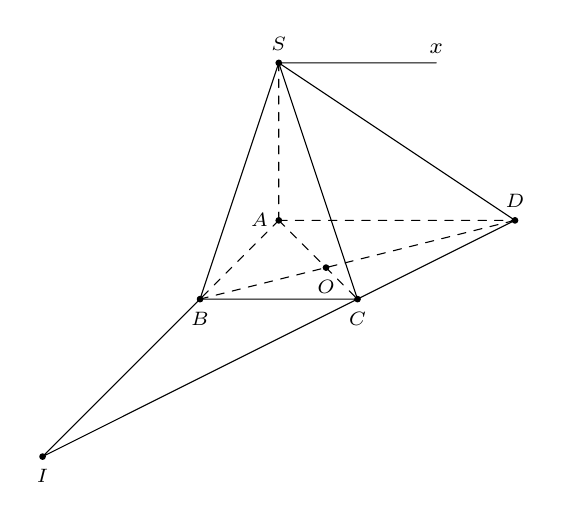
\begin{tikzpicture}[line join = round,line cap = round,>=stealth,font=\footnotesize,scale=1]
      \foreach \x/\y/\t in {0/0/A,3/0/D,-1/-1/B,1/-1/C,0/2/S,2/2/x}{
      \path (\x,\y) coordinate (\t); 
     } 
      \path
      (intersection of A--C  and B--D) coordinate (O)
      (intersection of D--C and B--A) coordinate  (I);
      \draw[dashed] (A)--(S)
      (A)--(B) 
       (A)--(D)
       (A)--(C)
       (B)--(D);
     \draw  (S)--(B)
       (S)--(C)
       (S)--(D)
      (B)--(C) 
      (C)--(D) 
       (S)--(x) node[above]{$x$}
      (B)--(I)--(C); 
     \foreach  \t/\g in {A/180,B/-90,C/-90,D/90,S/90,O/-90,I/-90}{
      \draw[fill=black] (\t) circle (1pt) node[shift={(\g:7pt)},font=\scriptsize]{$ \t  $};
     } 
    \end{tikzpicture}
  \end{center}
  \begin{itemchoice}
    \itemch{\bf Đúng.}\\
   Ta  có giao tuyến của $2$ mặt phẳng $(SAD)$ và $(SAB)$ là $SA$.
   \itemch{\bf  Sai.}\\
   Ta có $\heva{& AD\in (SAD) \\ & BC\in (SBC)\\ & S\in (SAD)\cap  (SBC)\\ & AD\parallel BC}\Rightarrow (SBC)\cap (SAD)=Sx\parallel AD\parallel BC$.
   \itemch{\bf Đúng.}\\ 
    Ta có giao tuyến của $2$ mặt phẳng $(SAC)$ và $(SBD)$ là đường thẳng $SO$, với $O=AC \cap BD$.
   \itemch{\bf  Đúng.}\\
   Vì $I=CD \cap AB$ nên giao điểm của $CD$ với mặt phẳng $(SAB)$  là $I$.
  \end{itemchoice}
 } 
\end{ex}

% nguồn: Ok_dungsai_lop11_Lan2
\begin{ex}%[1H4N4-1]%[ma:c963ee3c]
	Cho hai đường thẳng $a$ và $b$ nằm trong $(\alpha)$. Hai đường thẳng $a'$ và  $b'$ nằm trong mp $(\beta)$.
	\choiceTF 
		{Nếu $a\parallel a'$ và $b\parallel  b'$ thì $(\alpha)\parallel(\beta)$}
		{Nếu $(\alpha)\parallel(\beta)$ thì $a\parallel  a'$ và $b\parallel b'$}
		{Nếu $a\parallel b$ và $a'\parallel b'$  thì $(\alpha)\parallel(\beta)$}
		{\True Nếu $a$ cắt $b$, $a$ cắt  $b$ và $a\parallel a'$ và $b\parallel b'$ thì $(\alpha)\parallel(\beta)$}
	\loigiai{ 
		\begin{itemchoice}
			\itemch  \textbf{Sai}.\\
			Ta cần thêm ít nhất một trong hai dữ kiện $a$ và $b$  cắt nhau hoặc $a'$ và $b'$ cắt nhau.
			\itemch \textbf{Sai}.\\ 
			Các cặp đường thẳng này  có thể chéo nhau.
			\itemch \textbf{Sai}.\\ 
			$a$ với $b$ hoặc $a'$ với  $b'$ đều nằm chung trong một mặt phẳng nên không có mối liên hệ rõ ràng với mặt phẳng còn lại.
			\itemch \textbf{Đúng}.\\ 
			Theo dấu hiệu chứng minh hai mặt phẳng song song. 
		\end{itemchoice}
	} 
\end{ex}

% nguồn: Ok_dungsai_lop11_Lan2
\begin{ex}%[1H4N4-1]%[ma:f65cf5db]
	Cho hai mặt  phẳng phân biệt $(P)$ và $(Q)$.
	\choiceTF 
		{Nếu hai mặt phẳng $(P)$ và $(Q)$ song song với nhau thì  mọi đường thẳng nằm trên $(P)$ đều song song với mọi đường thẳng nằm trên $(Q)$}
		{\True Nếu mọi  đường thằng nằm trong mặt phẳng $(P)$ đều song song với $(Q)$ thì $(P)$ song song với $(Q)$}
		{\True Nếu hai mặt phẳng $(P)$ và $(Q)$ song song với nhau thì mọi đường thẳng nằm trên $(P)$ đều song  song với $(Q)$}
		 {Nếu mặt phẳng $(P)$ chứa hai đường thẳng cùng song song với $(Q)$ thì $(P)$ song song với $(Q)$}
	\loigiai{ 
		\begin{itemchoice}
			\itemch \textbf{Sai}.\\ Hai đường  thẳng đó có thể chéo nhau.
			 \itemch \textbf{Đúng}.
			 \itemch \textbf{Đúng}.
			\itemch \textbf{Sai}.\\ Thiếu dữ kiện hai đường thẳng đó còn phải cắt nhau. 
		\end{itemchoice}
	} 
\end{ex}

% nguồn: Ok_dungsai_lop11_Lan1
\begin{ex}%[1H4H4-1]%[ma:103531c3]
 Xét tính đúng/sai của các phát biểu  sau:
  \choiceTF
  {\True Qua một điểm nằm ngoài một mặt phẳng, tồn tại duy nhất một mặt phẳng song song với mặt phẳng đã cho} 
  {Hai mặt phẳng cùng song song  với một mặt phẳng thứ ba thì chúng song song với nhau}
  {\True Nếu hai mặt phẳng $(\alpha)$ và  $(\beta)$ song song với nhau thì mọi đường thẳng nằm trong $(\alpha)$ đều song song với $(\beta)$}
  {Nếu $\left(\alpha\right)\parallel a$ và $\left(\alpha\right)\parallel b$ với $a, b$ là hai đường  thẳng phân biệt thuộc $\left(\beta\right)$ thì mp $\left(\alpha\right)$ $\parallel$ mp $\left(\beta\right)$}
  \loigiai{
  \begin{itemchoice}
   \itemch Qua một điểm nằm ngoài một mặt phẳng, có một  và chỉ một mặt phẳng song song với mặt phẳng đó.
   \itemch Mệnh đề \lq\lq Hai mặt phẳng cùng song song với một mặt phẳng thứ ba thì chúng song song với nhau\rq \rq là một mệnh  đề sai vì hai mặt này có thể trùng nhau.
   \itemch Mệnh đề: \lq \lq Nếu hai mặt phẳng $(\alpha)$ và $(\beta)$ song song với nhau thì mọi đường thẳng nằm trong $(\alpha)$ đều song song  với $(\beta)$\rq \rq là đúng.
   \itemch Điều  kiện để mp $\left(\alpha\right)$ $\parallel$ mp $\left(\beta\right)$ là $\left(\alpha\right)\parallel a$ và $\left(\alpha\right)\parallel b$ với $a, b$ là hai đường thẳng \textbf{cắt nhau} thuộc $\left(\beta\right)$.
  \end{itemchoice}
 } 
\end{ex}

% nguồn: Ok_dungsai_lop11_Lan1
\begin{ex}%[1H4H4-1]%[ma:058b31dd]
 Cho biết tính đúng sai của mỗi phát  biểu sau?
 \choiceTF 
  {\True Hai mặt phẳng phân biệt không cắt nhau thì song  song}
  {Nếu mặt phẳng này chứa hai đường thẳng cùng song song với mặt phẳng kia thì hai mặt phẳng  đó song song với nhau}
  {Hai mặt phẳng cùng song song với mặt phẳng thứ ba thì  song song với nhau}
  {Hai mặt phẳng phân biệt cùng song song  với một đường thẳng thì song song với nhau}
  \loigiai{
  \begin{itemchoice}
   \itemch Đúng. 
   \itemch Sai. Vì trong  giả thiết đã thiếu đi một yếu tố cần thiết là hai đường thẳng phải cắt nhau, khi đó ta mới kết luận hai mặt phẳng song song với nhau.
   \itemch Sai. Vì hai mặt phẳng cùng song song  với mặt phẳng thứ ba thì chúng vẫn có thể trùng nhau.
   \itemch Sai. Vì hai mặt phẳng phân  biệt cùng song song với một đường thẳng thì chúng có thể cắt nhau hoặc song song với nhau.
  \end{itemchoice}
 } 
\end{ex}

% nguồn: Ok_dungsai_lop11_Lan1
\begin{ex}%[1H4V4-1]%[ma:23c5a721]
 Trong mặt phẳng $(P)$, cho hình bình hành $ABCD$. Vẽ các nửa đường thẳng song song nhau, nằm về  một phía đối với mặt phẳng $(P)$ và đi qua các điểm $A, B$, $C, D$. Một mặt phẳng $(Q)$ cắt bốn nửa đường thẳng nói trên tại $A'$, $B'$, $C'$, $D'$.
  \choiceTF
  {\True  ${mp}(AA',BB')$ song song với ${mp}(CC',DD')$}
   {\True $A'B'\parallel C'D'$}
  {Tứ giác $A'B'C'D'$ là hình thang} 
  {\True Gọi  $O$ và $O'$ lần lượt là giao điểm của hai đường chéo của $ABCD$ và $A'B'C'D'$. Khi đó $OO'\parallel AA'$}
  \loigiai{
  \begin{enumerate}
    \item Chứng minh ${mp}(AA',BB')$ và ${mp}(CC',DD')$ song song:\\
   Ta có $ AA'\parallel DD'$ và  $AB \parallel C D$ nên ${mp}(AA', BB')\parallel{mp}(CC', DD')$.
   \begin{center}
    \begin{tikzpicture}[scale=1,font=\footnotesize,line join=round,line cap=round,>=stealth]
      \def\bc{4} 
       \def\ba{2}
       \def\h{4}
      \def\gocB{35} 
       \coordinate[label=below left:$B$] (B) at (0,0);
      \coordinate[label=above left:$A$] (A) at (\gocB:\ba); 
      \coordinate[label=below:$C$] (C) at (\bc,0); 
       \coordinate[label=right:$D$] (D) at ($(C)-(B)+(A)$);
      \coordinate (H) at  ($(B)!0.4!(D)$);
      \coordinate[label=above left:$A'$] (A') at ($(H)+(90:\h)$); 
       \coordinate[label=left:$B'$] (B') at ($(B)-(A)+(A')$);
      \coordinate (C') at  ($(C)-(A)+(A')$);
      \coordinate  (D') at ($(D)-(A)+(A')$);
       \coordinate (a) at ($(A)!1.35!(A')$);
      \coordinate (b)  at ($(B)!1.35!(B')$);
      \coordinate [label=below right:$C'$](c) at ($(C)!0.75!(C')$); 
      \coordinate [label=right:$D'$](d) at ($(D)!0.75!(D')$); 
      \coordinate[label=below:$O$]  (O) at (intersection cs:first line={(A)--(C)},second line={(B)--(D)});
      \coordinate[label=above:$O'$] (O') at  (intersection cs:first line={(A')--(c)},second line={(B')--(d)});
       \draw (B')--(B)--(C)--(D)--(d)--(A')--(B')--(c)--(d)
       (C)--(C')
      (A')--(a) 
       (B')--(b)
      (C')--(c) 
      (D')--(d) 
      (B')--(d) 
       (A')--(c);
      \draw[dashed] (C)--(A)--(D)--(B) 
      (A')--(A)--(B) 
      (O)--(O'); 
      \foreach  \diem in {A,B,C,D,A',B',c,d,O,O'} \fill (\diem) circle (1pt);
     \end{tikzpicture}
   \end{center}
   \item Chứng minh  $A'B'C'D'$ là hình bình hành.\\
   Ta có $\heva{&{mp}(A A',BB')\parallel{mp}(CC',DD')\\ &(Q)\cap{mp}(AA',BB')=A'B'\\ &(Q)\cap{mp}(CC',DD')=C'D'}\Rightarrow A'B'\parallel  C'D'$.\quad (1)\\
   Hoàn toàn tương tự, ta chứng  minh được $A'D'\parallel B'C'$.\quad (2)
   \item Từ (1) và (2)  suy ra $A'B'C'D'$ là hình bình hành.
   \item Chứng  minh $O O'\parallel A A'$. \\
   Ta  có
    $$\heva{&(ACC'A')\cap(BDD'B')=OO'\\ &
   AA'\subset(ACC'A'), BB'\subset(BDD'B')\\  &
   AA'\parallel  BB'
   }\Rightarrow OO'\parallel AA'\parallel BB'\text{  hay }OO'\parallel AA'$$
  \end{enumerate}
  }
\end{ex}
